\chapter{GitHub Actions --- 自動化で開発を加速する}

\section{この章で学ぶこと}

この章では、GitHubに組み込まれた自動化プラットフォームである\textbf{GitHub Actions}について学びます。具体的には、以下の内容を扱います。

\begin{itemize}
  \item CI/CD（継続的インテグレーション/継続的デリバリー）とは何か、なぜ必要なのか
  \item GitHub Actionsを構成する基本用語（Workflow、Event、Job、Step、Action、Runner）
  \item YAMLファイルによるワークフローの定義方法を1行ずつ理解する
  \item トリガー（Event）の種類と使い分け
  \item Python、Node.js、自動リリースなど実用的なワークフロー例
  \item APIキーなどの秘密情報をワークフローで安全に扱う方法
  \item 料金体系と無料枠の制限
  \item ワークフローの実行結果の確認とデバッグ方法
\end{itemize}

「コードを書いたら、あとは自動でテスト・ビルド・デプロイしてほしい」――この願いを実現するのがGitHub Actionsです。

\section{CI/CDとは何か}

\subsection{手動テストの限界}

ソフトウェア開発の初期段階では、コードを変更するたびに手動でテストを実行し、問題がなければ手動でサーバーにデプロイする、というワークフローでも何とかなります。しかし、プロジェクトが成長し、チームメンバーが増え、1日に何度もコードが変更されるようになると、手動での確認は現実的ではなくなります。

たとえば、ある開発者がログイン機能を修正したとします。手動テストでは、ログイン機能自体が正しく動くかは確認できても、その変更が商品一覧ページや決済機能に影響を与えていないかまでは、なかなか確認しきれません。こうした「意図せず他の機能を壊してしまう」問題を\textbf{リグレッション（退行）}と呼びます。

\subsection{Continuous Integration（継続的インテグレーション）}

\textbf{CI（Continuous Integration）}とは、開発者がコードを共有リポジトリに統合（push/merge）するたびに、自動でビルドとテストを実行する手法です。「継続的」という言葉がついているのは、これを一度だけでなく、コードが変更されるたびに繰り返し行うためです。

CIを導入すると、以下のようなサイクルが自動的に回ります。

\begin{enumerate}
  \item 開発者がコードを変更してプッシュする
  \item CIシステムが自動的にテストを実行する
  \item テスト結果がPull Requestに表示される
  \item テストが通れば安心してマージできる。失敗すれば修正してから再挑戦する
\end{enumerate}

この仕組みがあることで、リグレッションを早期に発見でき、常にメインブランチが「動く状態」に保たれます。

\subsection{Continuous Delivery / Deployment（継続的デリバリー/デプロイ）}

\textbf{CD}はCIの延長にある概念で、テストに通ったコードを自動で本番環境にデプロイ（公開）する仕組みです。Continuous Deliveryは「いつでもデプロイ可能な状態を保つ」こと、Continuous Deploymentは「テストが通ったら自動的にデプロイまで行う」ことを指します。

GitHub Actionsは、このCI/CDの両方をGitHubの中で実現できるツールです。外部のCI/CDサービス（Jenkins、CircleCI、Travis CIなど）をわざわざ契約・設定する必要がなく、リポジトリの中にYAMLファイルを1つ置くだけで始められます。

\section{GitHub Actionsの基本用語}

GitHub Actionsを理解するには、6つの基本用語を押さえる必要があります。これらは相互に関係しているので、全体像を把握しながら1つずつ見ていきましょう。

\subsection{Workflow（ワークフロー）}

ワークフローは、自動化の全体を定義する\textbf{設計図}です。\cmd{.github/workflows/} ディレクトリに配置するYAMLファイル1つが、1つのワークフローに対応します。たとえば、テスト用のワークフロー（\cmd{ci.yml}）とデプロイ用のワークフロー（\cmd{deploy.yml}）を別々に作ることができます。

\subsection{Event（イベント）}

ワークフローを起動する\textbf{トリガー}です。「コードがプッシュされたら」「Pull Requestが作成されたら」「毎日午前0時になったら」など、さまざまな条件を指定できます。1つのワークフローに複数のイベントを設定することも可能です。

\subsection{Job（ジョブ）}

ワークフロー内で実行される\textbf{タスクの塊}です。1つのワークフローに複数のジョブを含めることができ、デフォルトでは各ジョブは\textbf{並列に}実行されます。ジョブ間に依存関係を設定すれば、「テストジョブが成功したらデプロイジョブを実行する」のように順序を制御できます。

\subsection{Step（ステップ）}

ジョブ内の\textbf{個々の処理}です。ステップは上から順に逐次実行されます。各ステップでは、シェルコマンドを実行するか、既存のActionを呼び出すかのいずれかを行います。

\subsection{Action（アクション）}

再利用可能な\textbf{処理の部品}です。GitHub Marketplaceには、コードのチェックアウト、言語のセットアップ、キャッシュの管理など、よく使う処理がActionとして公開されています。自分でゼロからスクリプトを書かなくても、\cmd{uses: actions/checkout@v4} のように参照するだけで利用できます。

\subsection{Runner（ランナー）}

ワークフローを実際に実行する\textbf{サーバー（仮想マシン）}です。GitHubが提供するRunner（GitHub-hosted runner）には、Ubuntu、macOS、Windowsの3種類があります。\cmd{runs-on: ubuntu-latest} のように指定します。自分のサーバーをRunnerとして使う「self-hosted runner」を設定することも可能です。

これらの関係を階層構造で整理すると、以下のようになります。

\begin{lstlisting}[language={}]
Workflow（YAMLファイル全体）
├── Event（トリガー: push, pull_request, schedule...）
├── Job 1（例: テスト）
│   ├── Step 1: actions/checkout を使ってコードを取得
│   ├── Step 2: actions/setup-python を使ってPythonをインストール
│   ├── Step 3: pip install で依存関係をインストール（run コマンド）
│   └── Step 4: pytest でテストを実行（run コマンド）
└── Job 2（例: デプロイ ← Job 1に依存）
    ├── Step 1: ビルド
    └── Step 2: デプロイ
\end{lstlisting}

\section{最初のワークフローを作ってみる}

ここでは、Pythonプロジェクトの簡単なCIワークフローを例に、YAMLファイルの各行が何を意味しているかを1つずつ解説します。

まず、リポジトリのルートに \cmd{.github/workflows/} ディレクトリを作成し、その中に \cmd{ci.yml} というファイルを作成します。

\begin{lstlisting}[language={}]
name: CI                          # (1) ワークフローの名前。Actions タブに表示される

on:                                # (2) トリガーの定義
  push:                            #     コードがプッシュされた時
    branches: [main]               #     main ブランチへのプッシュのみ対象
  pull_request:                    #     PRが作成・更新された時
    branches: [main]               #     main ブランチへのPRのみ対象

jobs:                              # (3) ジョブの定義
  test:                            # (4) ジョブ名（任意の名前）
    runs-on: ubuntu-latest         # (5) 実行環境（Ubuntu最新版のランナー）

    steps:                         # (6) ステップの定義
      - name: Checkout code        # (7) ステップ名（ログに表示される）
        uses: actions/checkout@v4  # (8) 公式Actionを使ってコードをチェックアウト

      - name: Setup Python
        uses: actions/setup-python@v5  # Pythonをインストールする公式Action
        with:                          # Actionに渡すパラメータ
          python-version: '3.12'       # Python 3.12を使用

      - name: Install dependencies
        run: pip install -r requirements.txt  # (9) シェルコマンドを直接実行

      - name: Run tests
        run: pytest                           # pytestでテストを実行
\end{lstlisting}

それぞれのポイントを補足します。

\textbf{(1) \cmd{name}} --- ワークフローの名前です。GitHub Actionsタブで一覧表示されるときに使われます。省略すると、ファイル名がそのまま表示されます。

\textbf{(2) \cmd{on}} --- 「いつこのワークフローを実行するか」を定義します。この例では、mainブランチへのpushと、mainブランチに対するPRが対象です。

\textbf{(5) \cmd{runs-on}} --- ジョブを実行するRunnerの種類です。\cmd{ubuntu-latest} を指定すると、GitHubが管理するUbuntuの最新LTS版が使われます。macOSが必要な場合は \cmd{macos-latest}、Windowsなら \cmd{windows-latest} を指定します。

\textbf{(8) \cmd{uses}} --- 既存のActionを利用する記法です。\cmd{actions/checkout@v4} は「GitHubの公式organizationが公開しているcheckoutアクションのv4」を意味します。\cmd{@v4} のようにバージョンを固定することで、Actionの更新による予期しない動作変更を防ぎます。

\textbf{(9) \cmd{run}} --- シェルコマンドを直接実行します。複数行のコマンドを書きたい場合は、パイプ記号 \cmd{|} を使います。

\begin{lstlisting}[language={}]
      - name: Install and test
        run: |
          pip install -r requirements.txt
          pytest --verbose
\end{lstlisting}

このファイルをリポジトリにプッシュするだけで、GitHub Actionsが自動的にワークフローを認識し、次回のpushやPR作成時にテストが実行されるようになります。

\begin{figure}[htbp]
\centering
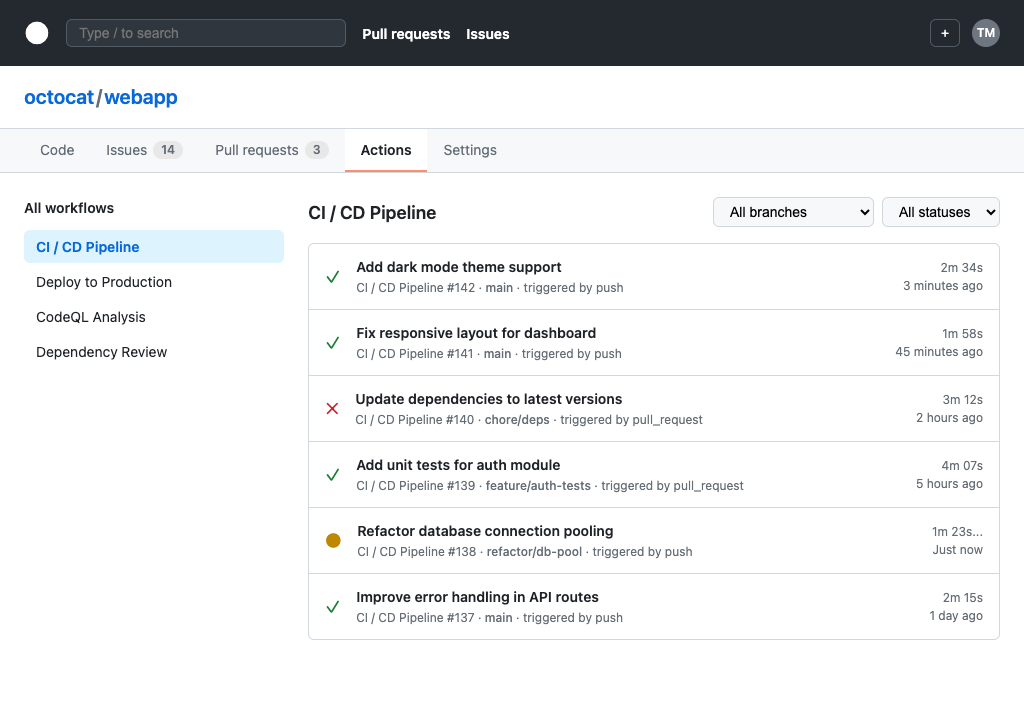
\includegraphics[width=0.95\textwidth]{images/actions-results.png}
\caption{GitHub Actionsタブでワークフローの実行結果が表示されている状態。緑のチェックマークが付いたジョブ一覧}
\end{figure}

\section{トリガー（Event）の種類}

ワークフローをいつ実行するかを決めるのがトリガーです。用途に応じてさまざまなトリガーが用意されています。

\subsection{push --- コードがプッシュされた時}

最も基本的なトリガーです。ブランチやファイルパスで条件を絞り込めます。

\begin{lstlisting}[language={}]
on:
  push:
    branches: [main, develop]      # mainまたはdevelopへのpush
    paths: ['src/**', 'tests/**']  # src/またはtests/配下の変更時のみ
\end{lstlisting}

\cmd{paths} フィルタは特に便利です。たとえば、ドキュメントだけを修正したのにテストが走るのは無駄です。\cmd{paths} でソースコードのディレクトリだけを指定しておけば、不要な実行を防げます。

\subsection{pull\_request --- Pull Requestに関するイベント}

\begin{lstlisting}[language={}]
on:
  pull_request:
    branches: [main]
    types: [opened, synchronize, reopened]  # PR作成時、更新時、再オープン時
\end{lstlisting}

\cmd{types} を省略すると、\cmd{opened}、\cmd{synchronize}、\cmd{reopened} がデフォルトで適用されます。

\subsection{schedule --- 定期実行}

cron式でスケジュール実行を設定できます。セキュリティスキャンや依存関係の更新チェックなど、定期的に行いたいタスクに適しています。

\begin{lstlisting}[language={}]
on:
  schedule:
    - cron: '0 0 * * *'   # 毎日UTC 0時（日本時間 午前9時）
    - cron: '0 9 * * 1'   # 毎週月曜UTC 9時
\end{lstlisting}

cron式の各フィールドは左から「分 時 日 月 曜日」です。時刻はUTC基準であることに注意してください。

\subsection{workflow\_dispatch --- 手動実行}

ボタン1つでワークフローを手動実行できるトリガーです。入力パラメータを定義すると、実行時にドロップダウンやテキストフィールドで値を指定できます。

\begin{lstlisting}[language={}]
on:
  workflow_dispatch:
    inputs:
      environment:
        description: 'デプロイ先の環境'
        required: true
        default: 'staging'
        type: choice
        options:
          - staging
          - production
      dry_run:
        description: 'ドライランモード（実際にはデプロイしない）'
        required: false
        type: boolean
        default: true
\end{lstlisting}

\begin{figure}[htbp]
\centering
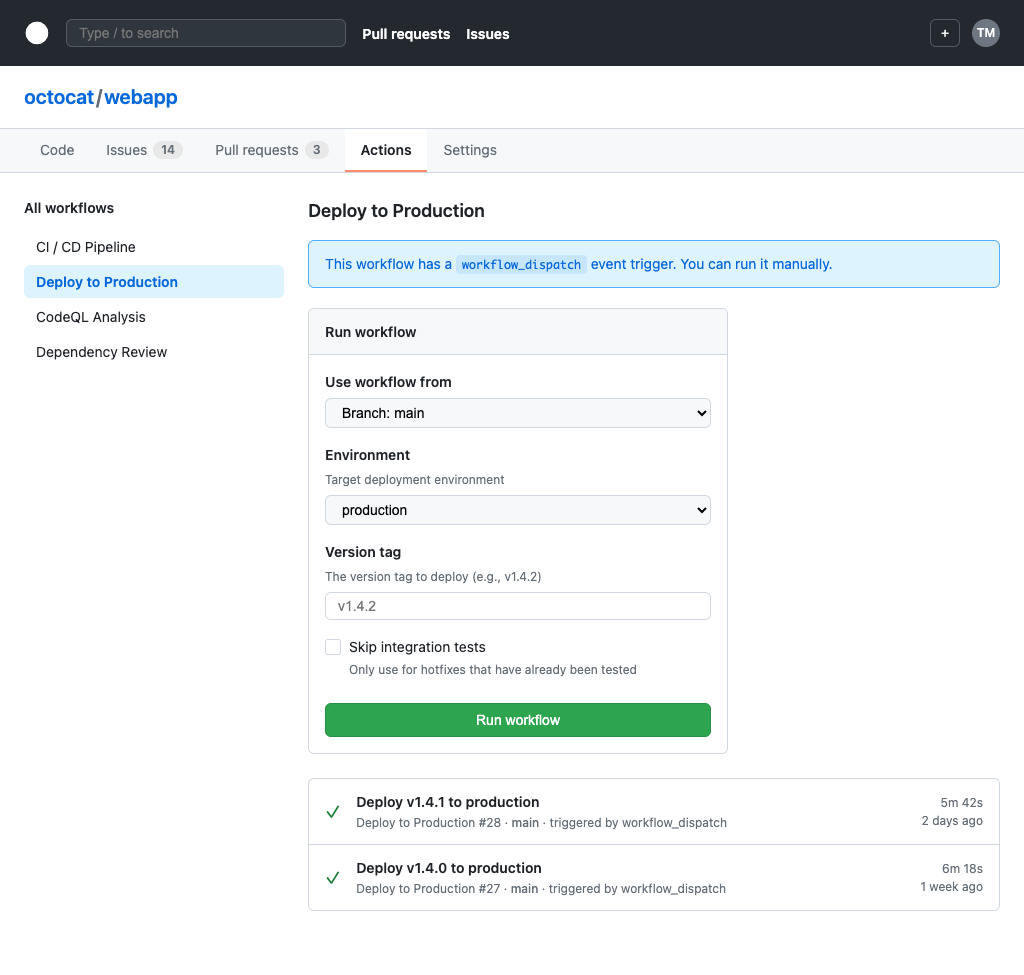
\includegraphics[width=0.95\textwidth]{images/actions-workflow-dispatch.png}
\caption{workflow\_dispatchの手動実行画面。入力フィールドとRun workflowボタンが表示されている状態}
\end{figure}

\subsection{release --- リリース公開時}

\begin{lstlisting}[language={}]
on:
  release:
    types: [published]  # リリースが公開された時
\end{lstlisting}

このトリガーは、第14章で学ぶリリース機能と組み合わせて、バイナリの自動ビルドやパッケージの自動公開に使われます。

\section{実用的なワークフロー例}

\subsection{Pythonプロジェクトの本格的なCI}

複数のPythonバージョンでテストを実行し、リンターによるコード品質チェックも行う例です。\cmd{strategy.matrix} を使うと、指定した組み合わせのすべてに対してジョブが自動的に実行されます。

\begin{lstlisting}[language={}]
name: Python CI

on:
  push:
    branches: [main]
  pull_request:
    branches: [main]

jobs:
  test:
    runs-on: ubuntu-latest
    strategy:
      matrix:
        python-version: ['3.10', '3.11', '3.12']  # 3バージョンでテスト

    steps:
      - uses: actions/checkout@v4

      - name: Setup Python ${{ matrix.python-version }}
        uses: actions/setup-python@v5
        with:
          python-version: ${{ matrix.python-version }}

      - name: Cache pip
        uses: actions/cache@v4
        with:
          path: ~/.cache/pip
          key: ${{ runner.os }}-pip-${{ hashFiles('requirements.txt') }}

      - name: Install dependencies
        run: |
          python -m pip install --upgrade pip
          pip install -r requirements.txt

      - name: Lint with ruff
        run: ruff check .

      - name: Test with pytest
        run: pytest --cov=src --cov-report=xml

      - name: Upload coverage
        uses: codecov/codecov-action@v4
\end{lstlisting}

\cmd{actions/cache@v4} はビルド時間を短縮するための重要なActionです。\cmd{requirements.txt} が変わらない限り、前回インストールしたパッケージのキャッシュが再利用されます。大規模なプロジェクトでは、キャッシュの有無でビルド時間が数分変わることもあります。

\subsection{Node.jsプロジェクトのCI}

\begin{lstlisting}[language={}]
name: Node.js CI

on:
  push:
    branches: [main]
  pull_request:
    branches: [main]

jobs:
  build:
    runs-on: ubuntu-latest

    steps:
      - uses: actions/checkout@v4

      - name: Setup Node.js
        uses: actions/setup-node@v4
        with:
          node-version: '20'
          cache: 'npm'          # npm のキャッシュを自動管理

      - name: Install dependencies
        run: npm ci             # npm install より厳密で高速

      - name: Lint
        run: npm run lint

      - name: Test
        run: npm test

      - name: Build
        run: npm run build
\end{lstlisting}

\cmd{npm ci} は \cmd{npm install} と異なり、\cmd{package-lock.json} に基づいて厳密にパッケージをインストールします。CI環境では、環境ごとにバージョンが異なるという問題を防ぐために \cmd{npm ci} が推奨されます。

\subsection{タグプッシュによる自動リリース}

\begin{lstlisting}[language={}]
name: Release

on:
  push:
    tags: ['v*']          # v で始まるタグがプッシュされた時

jobs:
  release:
    runs-on: ubuntu-latest
    permissions:
      contents: write     # リリース作成に必要な権限

    steps:
      - uses: actions/checkout@v4

      - name: Create Release
        uses: softprops/action-gh-release@v2
        with:
          generate_release_notes: true  # PRラベルから自動でリリースノート生成
\end{lstlisting}

\section{Secrets（シークレット）}

\subsection{なぜSecretsが必要か}

ワークフローの中で外部サービスのAPIキーやデプロイ用のパスワードを使いたい場面があります。しかし、これらの秘密情報をYAMLファイルに直接書いてしまうと、リポジトリにアクセスできる全員に見えてしまいます。パブリックリポジトリの場合は、世界中の誰からも見える状態になります。

GitHub Secretsは、こうした秘密情報を\textbf{暗号化して安全に保存}し、ワークフローの中からだけ参照できるようにする仕組みです。Secretsの値はログに出力される場合も自動的に \cmd{***} にマスクされるため、誤って表示されることはありません。

\subsection{Secretsの設定方法}

Web UIでは、リポジトリの Settings → Secrets and variables → Actions → 「New repository secret」から設定します。

\begin{figure}[htbp]
\centering
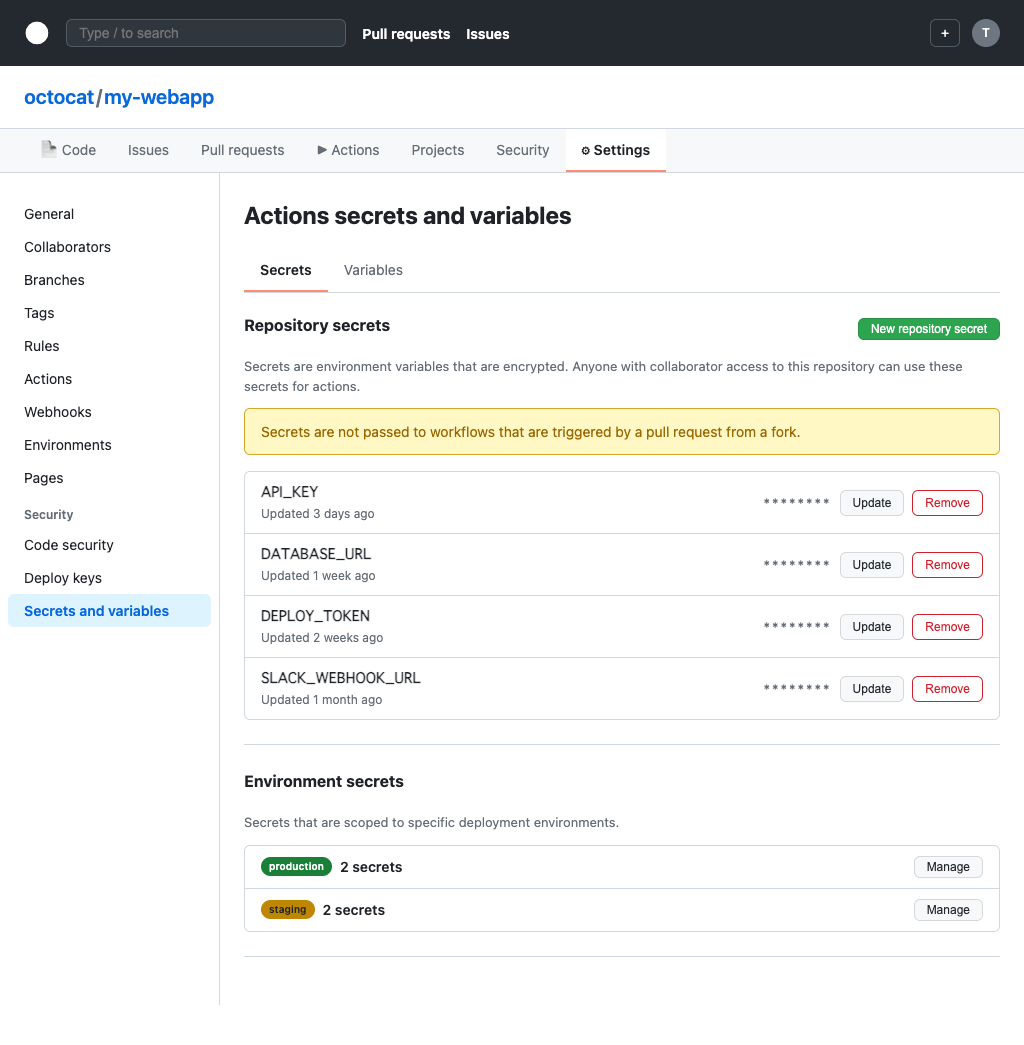
\includegraphics[width=0.95\textwidth]{images/secrets-settings.png}
\caption{リポジトリのSecrets設定画面。シークレット名の一覧が表示されている状態（値は表示されない）}
\end{figure}

CLIからも設定できます。

\begin{lstlisting}[language=bash]
# 対話的に値を入力（画面に表示されない）
gh secret set API_KEY

# ファイルから値を読み込む
gh secret set API_KEY < api_key.txt

# 環境変数から設定
echo "$MY_API_KEY" | gh secret set API_KEY
\end{lstlisting}

一度設定したSecretの値は、Web UIからもCLIからも\textbf{読み取ることはできません}。値を確認したい場合は、再度設定し直す必要があります。これはセキュリティ上の意図的な設計です。

\subsection{ワークフローでの使い方}

Secretsはワークフロー内で \cmd{\$\{\{ secrets.SECRET\_NAME \}\}} という構文で参照します。

\begin{lstlisting}[language={}]
steps:
  - name: Deploy to production
    env:
      API_KEY: ${{ secrets.API_KEY }}
      DEPLOY_TOKEN: ${{ secrets.DEPLOY_TOKEN }}
    run: |
      echo "Deploying with API key..."
      ./deploy.sh
\end{lstlisting}

\cmd{env} でシェルの環境変数にマッピングしてからスクリプト内で使うのが一般的なパターンです。\cmd{\$\{\{ secrets.API\_KEY \}\}} を \cmd{run} の中に直接書くこともできますが、\cmd{env} を使うほうがスクリプトの可読性が高く、別環境での再利用もしやすくなります。

\section{料金と制限}

GitHub Actionsの料金は、リポジトリの種類とRunnerのOSによって異なります。

\subsection{パブリックリポジトリ}

パブリックリポジトリでは、GitHub Actionsは\textbf{完全に無料}で、実行時間の制限もありません。これはオープンソースプロジェクトにとって非常に大きなメリットです。

\subsection{プライベートリポジトリ}

プライベートリポジトリでは、プランに応じた月間の無料枠が設けられています。

\begin{tabular}{|l|l|l|l|}
\hline
\textbf{プラン} & \textbf{Linux} & \textbf{macOS} & \textbf{Windows} \\
\hline
Free & 2,000分/月 & 200分/月 & 500分/月 \\
\hline
Pro & 3,000分/月 & 300分/月 & 750分/月 \\
\hline
Team & 3,000分/月 & 300分/月 & 750分/月 \\
\hline
Enterprise & 50,000分/月 & 5,000分/月 & 10,000分/月 \\
\hline
\end{tabular}

注意すべき点として、macOSランナーはLinuxランナーの\textbf{10倍}の分数として計算されます。つまり、macOSで10分間実行すると、Linuxの100分ぶんに相当します。Windowsは2倍です。特別な理由がなければ、\cmd{runs-on: ubuntu-latest} を使用することでコストを抑えられます。

無料枠を超過した場合は追加料金が発生しますが、デフォルトでは支出制限が\$0に設定されているため、意図せず高額な請求が来ることはありません。ただし、設定を変更している場合は注意が必要です。

\subsection{その他の制限}

\begin{itemize}
  \item ワークフロー1回の実行時間: 最大\textbf{6時間}（ジョブ単位）
  \item ワークフローの同時実行数: プランにより異なる
  \item APIリクエスト: 1時間あたり1,000リクエスト
\end{itemize}

\section{ワークフローの確認とデバッグ}

\subsection{CLIでの操作}

ワークフローの実行結果は、Web UIのActionsタブで確認できますが、CLIでもすべての操作が可能です。

\begin{lstlisting}[language=bash]
# 最近のワークフロー実行一覧を表示
gh run list

# 特定のワークフローだけ表示
gh run list --workflow ci.yml

# 実行の詳細を確認（各ステップの成否が分かる）
gh run view 1234567890

# ログを表示（エラーの原因を調査する際に必須）
gh run view 1234567890 --log

# 失敗したステップのログだけ表示
gh run view 1234567890 --log-failed

# 失敗したワークフローを再実行
gh run rerun 1234567890

# 失敗したジョブだけ再実行（時間短縮）
gh run rerun 1234567890 --failed

# ワークフローの実行をブラウザで確認
gh run view 1234567890 --web
\end{lstlisting}

\begin{figure}[htbp]
\centering
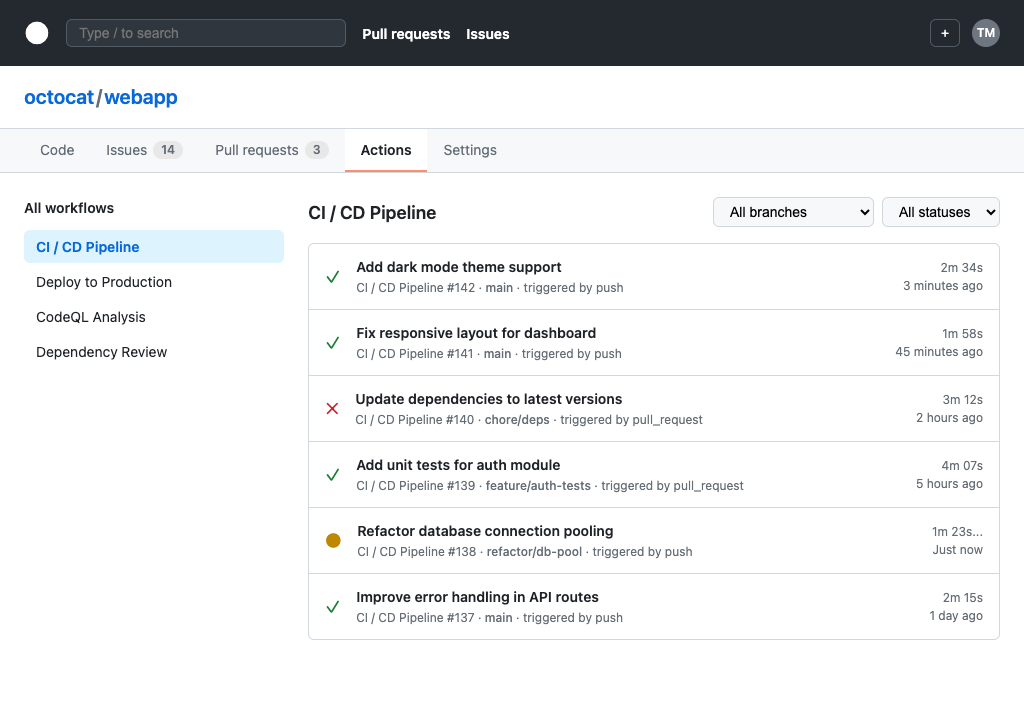
\includegraphics[width=0.95\textwidth]{images/actions-results.png}
\caption{GitHub ActionsタブでCIワークフローの実行結果が表示されている状態。各ステップの実行時間と成否が確認できる}
\end{figure}

\subsection{デバッグのコツ}

ワークフローが失敗した場合、まずは \cmd{--log-failed} でエラーログを確認しましょう。よくある失敗の原因には以下のようなものがあります。

\begin{itemize}
  \item \textbf{依存関係のインストール失敗} --- \cmd{requirements.txt} や \cmd{package.json} に存在しないパッケージが指定されている
  \item \textbf{テストの失敗} --- コードのバグ。ローカルで再現してから修正する
  \item \textbf{権限の不足} --- \cmd{permissions} の設定が不足している（特にリリース作成やPages デプロイ時）
  \item \textbf{Secretsの未設定} --- 必要なSecretが設定されていない（Secret名のtypoにも注意）
\end{itemize}

ワークフローの開発中にデバッグ用のステップを追加することもできます。

\begin{lstlisting}[language={}]
      - name: Debug info
        run: |
          echo "Runner OS: $RUNNER_OS"
          echo "Working directory: $(pwd)"
          ls -la
          python --version
\end{lstlisting}

ただし、Secretsの値をデバッグ用にechoすると自動的にマスクされるため、値そのものは確認できません。

\section{まとめ}

この章では、GitHub Actionsによるワークフロー自動化の基礎から実践までを学びました。

\begin{itemize}
  \item \textbf{CI/CD}は、コード変更のたびに自動でテスト・ビルド・デプロイを行う手法であり、ソフトウェアの品質を維持しながら開発速度を上げるために不可欠です
  \item GitHub Actionsは\textbf{Workflow、Event、Job、Step、Action、Runner}の6つの概念で構成されており、\cmd{.github/workflows/} ディレクトリにYAMLファイルを置くだけで利用できます
  \item \textbf{トリガー}には push、pull\_request、schedule、workflow\_dispatch などがあり、用途に応じて適切なものを選択します
  \item \cmd{strategy.matrix} を使えば、複数のバージョンや環境での\textbf{マトリクステスト}が簡単に設定できます
  \item \textbf{Secrets}を使うことで、APIキーやパスワードなどの秘密情報をワークフロー内で安全に利用できます
  \item パブリックリポジトリでは\textbf{無料・無制限}、プライベートリポジトリでもプランに応じた無料枠があります
\end{itemize}

GitHub Actionsは、最初の設定こそYAMLの記法に慣れる必要がありますが、一度設定してしまえば、その後のすべてのpushやPRに対して自動的にテストが走り、チーム全体の開発効率が大きく向上します。「まずは簡単なテスト実行から始めて、徐々にワークフローを充実させていく」というアプローチが、導入を成功させるコツです。
